\documentclass[a4paper,11pt]{article}
\usepackage{sbpo-template}
\usepackage[english]{babel}%brazil
%eu que inseri o pacote t1 fontenc
\usepackage[T1]{fontenc}
\usepackage[utf8]{inputenc} %latin1
\usepackage{amsmath,amssymb}
\usepackage{url}
\usepackage{graphicx}
\usepackage[caption=false]{subfig}
\usepackage{braket}
\usepackage{amsfonts}
\usepackage{amsthm}
\usepackage{fancyhdr}
\usepackage{comment}
\usepackage{float}
\usepackage{mathtools}
\usepackage{xspace}
\usepackage[inline]{enumitem}
\usepackage[export]{adjustbox}

 %\usepackage{subfigure}
%\usepackage{subcaption}
%\usepackage[subfigure]{tocloft}
%\usepackage[subfigure]{tocloft} 
%\usepackage{subfigure} 
\usepackage{marginnote}
\usepackage[usenames, dvipsnames]{color}
\usepackage[nameinlink, nosort]{cleveref}

\usepackage[square]{natbib}
\usepackage{indentfirst}

\title{The Complexity of $B_{1}$-EPG-Helly Graph Recognition} 

\newtheorem{theorem}{Theorem}
\newtheorem{lema}[theorem]{Lemma}
\newtheorem{defi}[theorem]{Definition}
\newtheorem{coro}[theorem]{Corollary}
\newtheorem{prop}[theorem]{Proposition}
\renewcommand{\proofname}{Proof}

\newcommand\floor[1]{\left\lfloor #1 \right\rfloor}
\newcommand\toricclass[1]{#1_\circ^\circ}
\newcommand{\toric}[1]{\left[#1\right]^\circ_\circ}
\renewcommand\mod[1]{\!\!\!\!\!\pmod{#1}}

\hyphenation{re-pre-sen-ta-ção}
\begin{document}

\pagestyle{fancy}

\maketitle
\if 10

\author{ 
\name{Claudson Bornstein}
\institute{Filia\c c\~ao} 
\iaddress{Endere\c co da Institui\c c\~ao}
\email {e-mail}
}

\author{
\name{Tanilson Santos}
\institute{Universidade Federal do Rio de Janeiro - UFRJ}
\iaddress{Endere\c co da Institui\c c\~ao}
\email{tanilson$@$cos.ufrj.br}
}

\author{ 
\name{Uéverton Souza}
\institute{Universidade Federal do Fluminense - UFF} 
\iaddress{Endere\c co da Institui\c c\~ao}
\email {e-mail}
}

\author{ 
\name{Jayme Szwarcfiter}
\institute{Filia\c c\~ao} 
\iaddress{Endere\c co da Institui\c c\~ao}
\email {e-mail}
}

\fi

% \vspace{8mm}
% \begin{resumo}
% Golumbic, Lipshteyn e Stern definiram em 2009 os grafos EPG, uma classe de grafos de intersecção baseada na intersecção de arestas de caminhos em uma grade. Um grafo EPG $G$ é um grafo que admite um esquema de representação onde seus vértices são representados por caminhos de uma grade $Q$, de tal forma que dois vértices em $G$ são adjacentes se e somente se seus caminhos correspondentes em $Q$ possuem arestas em comum. Quando tais caminhos em $Q$ possuem no máximo $k$ mudanças de direção (dobras), dizemos que esta é uma representação $B_k$-EPG.
% Uma coleção $C$ de conjuntos satisfaz a propriedade Helly quando toda subcoleção de $C$ que é mutuamente intersectante possui pelo menos um elemento comum. Neste trabalho mostramos que o reconhecimento de grafos que admitem representação $B_1$-EPG satisfazendo a propriedade Helly é NP-difícil.
% \end{resumo}
% \bigskip
% \begin{palchaves}
% EPG, grafos de intersecção, Helly, dobra simples, NP-difícil.

% \bigskip
% \noindent{TAG - Teoria e Algoritmos em Grafos}
% \end{palchaves}


\vspace{8mm}

\begin{abstract}
Golumbic, Lipshteyn and Stern defined in 2009 the class of EPG graphs, an intersection graph class  based on edge intersection of paths on a grid. An EPG graph $G$ is a graph that admits a representation where its vertices correspond to paths in a grid $Q$, such that two vertices of $G$ are adjacent if and only if their corresponding paths in $Q$ have a common edge. If the paths in $Q$ have at most $k$ changes of direction  (bends), we say that this is a  $B_k$-EPG representation. A collection $C$ of sets satisfies the Helly property when every sub-collection of $C$ that is pairwise intersecting has at least a common element. In this paper we show that the problem of recognizing $B_1$-EPG graphs that satisfy the Helly property is NP-complete.  
%Golumbic, Lipshteyn e Stern have defined in 2009 the EPG graphs, a intersection graph class  based in edge intersection of paths into a grid. A EPG graph $G$ is a graph that admits a representation scheme where its vertices are represented by paths in a grid $Q$, such that two vertices in $G$ are adjacent if and only if their corresponding paths in $Q$ have a common edge. When these paths in $Q$ have maximum $k$ changes of direction  (bends), we say that this is a  $B_k$-EPG representation. A colection $C$ of sets satisfies the Helly property when every sub-collection of $C$ that is mutually intersecting has at least a common element. In this paper we show that the problem of recognizing $B_1$-EPG graphs that satisfy the Helly property is NP-hard.      

%Edge-intersection graphs of Paths on a Grid (EPG) is a class that has been defined by \cite{golumbic2009}, in which represented vertices as paths and  the intersection of theses paths is different from empty if and only if the corresponding vertices are adjacent. When every path representation has at most $k$ bends, then we say this graph has a \textit{$ B_k-$EPG} representation. When $k = 1$ it has \textit{single bend} representation. %

%A family of sets is \textit{mutually intersecting} if given any two sets of the family, they intersect. A colection $C$ satisfies the \textit{Helly property} when every subcolection $C$ that is intercecting has at least one element  common.

%The class of EPG graphs has been studied by several researchers, such as \cite{ries2009}, \cite{alcon2016}, \cite{Asinowski2009} and others. 

%Despite the efforts of the scientific community, few problems in EPG graphs class are classified.
%The Helly property can be applied to the single bend representation problem, i.e. $B_1$-EPG-Helly. The recognizing of these graphs was open. 
%The prove of $NP-$completness to $B_1-$EPG-Helly is a non-trivial reduction. Our demonstration is based on the paper of~\cite{heldt2014}. %It is easy verify a single bend helly representation of any graph in polynomial time, so $B_1-$EPG-Helly Recognittion is in NP. 
%For NP-hardness we set up a reduction from problem One-In-Three 3SAT, with positive variables.%, known as NP-complete.%, Johnson~\cite{johnson1979}.%, [L04] problem. 
%The One-In-Three 3SAT problem consists in given a set $U$ of variables, collection $C$ of clauses over $U$ such that each clause $c \in C$ has $|c|=3$, answer the following question: Is there a truth assignment for $U$ such that each clause in $C$ has exactly one true literal?

%\cite{heldt2014} has demonstrated that recognizing $B_1$-EPG is NP-complete. Our paper show that recognizing $B_1$-EPG-Helly graphs might also be NP-complete. %, and our demonstration on $B_1$-EPG-Helly was the first subclass of $B_1$-EPG shown to be $NP$-complete. This we believe that recognizing $B_k$-EPG problem might also be $NP$-complete.

\end{abstract}

\bigskip
\begin{keywords}
EPG, Intersection Graphs, Helly, Single Bend, NP-completeness.

\bigskip
\noindent{TAG - Theory and Graph algorithms}
\end{keywords}

\newpage

\section{Introduction}

An EPG graph $G$ is a graph that admits a representation in which its vertices are represented by paths of a grid $Q$, such that two vertices of $G$ are adjacent if and only the corresponding paths have at least a common edge. The study of EPG graphs has practical motivation related to the problem of layout of digital circuits, which can be represented as paths in a rectangular orthogonal grid.

Every graph $G$ has an EPG representation, see~\citep{golumbic2009}. A graph has a $ B_k$-EPG representation if there is a representation for the graph in which each path has at most $k$ bends.


For some classes of graphs we known the smallest value of $k$ for witch the graphs in the class are $B_k$-EPG, such as interval graphs which coincide
 with $B_0$-EPG; the class of trees, which are in $ B_1$-EPG; the class of the outerplanar graphs, which are in $B_2$-EPG; and the class of planar graphs which are in $ B_4 $-EPG.

The class of EPG graphs has been studied by several researchers, such as \citep{ries2009, alcon2016, cohen2014}, among others. The investigations frequently approach characterizations with respect to the number of bends of the graph representation. Regarding the complexity of recognition, only the complexity of 3 sub-classes of EPG graphs have been determined: $ B_0$-EPG, $ B_1$-EPG ~\citep{heldt2014} and more recently $B_2$-EPG ~\citep {martin2017}, and only $ B_0$-EPG can be recognized in polynomial time, because it corresponds to the class of interval graph, see ~\citep{booth1976}. As an example, the Figure~\ref{fig:trianguloepgRepresentacao}(a) shows a $C_3$ graph, in the Figure~\ref{fig:trianguloepgRepresentacao}(b) we have an EPG representation where the paths do not have bend, in  the Figure~\ref{fig:trianguloepgRepresentacao}(c) show a representation with 1 bend and in the Figure~~\ref{fig:trianguloepgRepresentacao}(d) a representation where every path has at most 2 bends.

\begin{figure}[h]
  %\centering
  \begin{tabular}{ p{2.5cm} p{2.6cm} p{3.7cm} p{2.5cm} }
     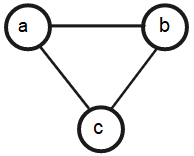
\includegraphics[width=2.3cm, left]{./img/trianguloabc.png} & 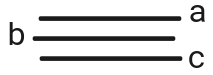
\includegraphics[width=2.5cm]{./img/b0epgtriangulo.png} & 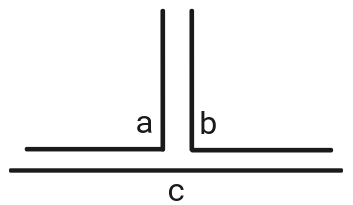
\includegraphics[width=3.5cm, left]{./img/b1epgtriangulo.png} & 
  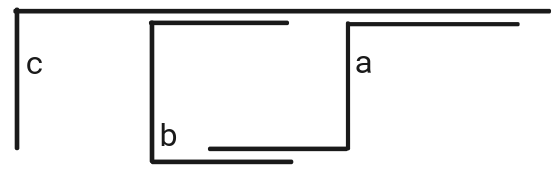
\includegraphics[width=5cm]{./img/b2epgtriangulo.png}\\%[\abovecaptionskip]
    \footnotesize (a) The $C_3$ graph & \footnotesize(b) $B_0$-EPG representation of $C_3$  & \footnotesize \centering (c) $B_1$-EPG representation of $C_3$  &  \footnotesize  (d) $B_2$-EPG representation of $C_3$ \\
 %\footnotesize & \footnotesize \centering representation & \centering  \footnotesize representation  & \footnotesize \centering representation\\  
  \end{tabular}
  %\vspace{2cm}  
%segundo bloco de figuras
%   \begin{tabular}{r p{2.5cm} @{}c@{} }
%     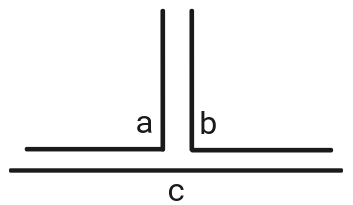
\includegraphics[width=4cm]{./img/b1epgtriangulo.png} & &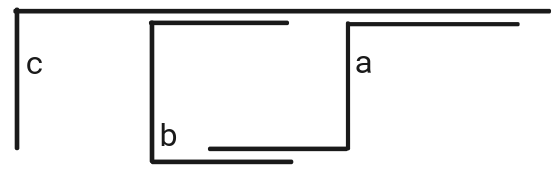
\includegraphics[width=6cm]{./img/b2epgtriangulo.png}  \\%[\abovecaptionskip] 
%     \footnotesize (c) Representação $B_1$-EPG($C_3$) & & \footnotesize (d) Representação $B_2$-EPG($C_3$)
%   \end{tabular}
 \caption{The $ C_3 $ graph  and some representations: without bend, with 1 bend and with 2 bends} \label{fig:trianguloepgRepresentacao}
\end{figure}

%Uma coleção $C$ de conjuntos é Helly quando toda subcoleção de $C$ que é mutuamente intersectante possui pelo menos um elemento comum.

A  collection $C$ of sets satisfies the Helly property when every sub-collection of $ C $ that is pairwise intersecting has at least one common element. The Helly property has this name in honor of the great Austrian mathematician Eduard Helly, who in 1923 proposed his famous theorem concerning the relation of intersecting sets.

The study of the Helly property is useful in the most diverse areas of science, and we can enumerate applications in semantics, code theory, computational biology, database, image processing, graph theory, optimization, and linear programming \citep{dourado2009}.% \ citep {teles2016}.


Note that the representation of Figure~\ref{fig:trianguloepgRepresentacao}(b) satisfies the Helly property, while the representations of Figures~\ref{fig:trianguloepgRepresentacao}(c) and~\ref{fig:trianguloepgRepresentacao}(d) do not satisfy it.


This paper studies graphs that have Helly EPG representation. Our contribution will be present a proof of NP-completeness related to the $ B_1$-EPG-Helly recognition problem.% whose representation has the Helly property.

   %@comment retirado para o SBPO
   %Dessa forma, para situar o leitor neste contexto, são definidos na seção seguinte os principais termos utilizados ao longo deste escrito. 
 
 
 \subsection{Basic definitions}

%@comment falar q a diagonal não é considerada
%ver se o conceito de direção não confunde com caminho direcionado

The term \emph{grid} is used to denote the Euclidean space of integers orthogonal coordinates. Each pair of integers corresponds to a pair of \emph{coordinates},  when convenient we will call as \emph {vertex of the grid}. The term \emph{edge of the grid}, will be used to denote a pair of coordinates that are at a distance one. Two edges $e_1$ and $e_2$ are \emph{consecutive edges} whether they have a common vertex. %A \emph{finite sequence of consecutive edges} is a finite sequence where every vertices are differents  
A \emph{path in the grid} is any finite sequence of consecutive edges, without vertex repetition, of the grid.
An edge is vertical when the first coordinate of the vertices composing it are equal, it is horizontal otherwise. A \emph {bend} in a path is a pair of consecutive edges $ e_1, e_2 $ of that path, such that $ e_1$'s direction is different from $ e_2$'s direction. A \emph {grid segment} is a path with no bends. Two paths are said to be \emph{edge-intersecting}, or for simplicity  intersecting, if they share at least one edge of the grid. Otherwise we say they are \emph{edge-disjoint} (or disjoint).

EPG is an acronym used to denote a class of intersection graphs based on the edge intersection of paths in a grid. This class, defined in 2009~\citep{golumbic2009}, consists of the class of graphs that allows a representation scheme where its vertices are represented by paths of a grid $ Q $, such that two vertices in $ G $ are adjacent if and only if its corresponding paths in $ Q $ intersect. If every path in a representation can be represented with at most $ k $ bends, we say that this graph $ G $ has a \emph{ $ B_k$-EPG} representation.%, and we will indicate this representation by the notation $ B_k$-EPG($ G $).
When $ k = 1 $ we say that this is a \emph{single bend} representation.


%Two sets, $ A $ and $ B $, are \emph{intersecting} $ A \cap B \neq \emptyset $. 
A family of sets is said to be pairwise intersecting if given any two sets of the family, they intersect. A collection of non-empty sets $C$ satisfies the Helly property when every pairwise intersecting sub-collection of $ C $ has one element that is in every subset of $C$.

The Helly property, can be applied to the $ B_k $-EPG representation problem, where each path is considered a set of edges. A graph $ G $ has a  $ B_k$-EPG-Helly representation if there is a representation for this graph where each path, which represents a vertex of the graph $ G $, has at most $ k $ bends and this representation satisfies the Helly property. Further for all subset of pairwise intersecting paths, there is an edge common to all paths of this subset, we will indicate this representation by the notation H-$B_k$-EPG($G$). The Figure~\ref{fig:triangulos} presents two $B_1$-EPG representations of a complete graph with three vertices. In Figure~\ref{fig:triangulos}(a), although the three paths are pairwise intersecting, there is no edge in all 3 paths, and therefore they do not satisfy the Helly property. The Figure~ \ref{fig:triangulos}(b) presents 3 pairwise intersecting paths, containing a common edge to the paths, so it is a valid $ B_1$-EPG-Helly representation.

\begin{figure}[h]
  \centering
  \begin{tabular}{p{3.7cm} p{1.5cm} p{3.3cm}}
     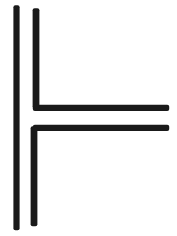
\includegraphics[width=1.8cm, center]{./img/1.png} & &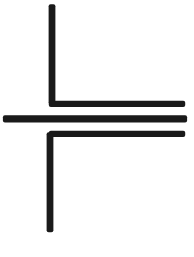
\includegraphics[width=1.8cm, center]{./img/2.png}  \\%[\abovecaptionskip]
    \footnotesize (a) Non-Helly representation (\textit{cross clique}) & & \footnotesize (b) Helly representation (\textit{line clique})%\\
 %   &&
  \end{tabular}
 \caption{$B_{1}$-EPG representations of the cycle of size 3}\label{fig:triangulos}
\end{figure}
  

An \emph{edge (of the grid) is relevant} if at least one of its coordinates is start, bend, or end of a path. A  \emph{maximal segment} is one whose its ends are relevants edges.  

A maximal segment $s$ of a path $p$ in a $B_k$-EPG representation that has no adjacency and only one of its ends is not bend, we say that this path has an \emph{optional bend}.   

%When every edge of each path end that has not adjacency is iteratively removed of the representation keeping adjacencies among paths, so that if the representation was Helly, it remains Helly.

A $B_k$-EPG representation \emph{was minimized} when all columns $(i,i+1)$ and lines $(j,j+1)$ that have only not relevant edges in the representation are removed. This process gives it back a minimal representation (in grid space, i.e. a representation in polynomial space)  without using unnecessary spaces. 

When the $B_k$-EPG representation was minimized and it does not have optional bends we say that this $B_k$-EPG representation is minimal.


In a $B_k$-EPG representation when the ends of a path $p$ are obstructed, i.e. another path $q$ can not be intersecting only the $p$ by the ends of $p$, then we have a situation of \emph{obstructed end}. If this situation occurs in a bend, then we say that there is a \emph{obstructed bend}.
 
 \begin{lema} \citep{golumbic2009} \label{lem:todoGrafoEpg}
 Every graph is EPG.
 \end{lema}
 \begin{proof}
 Let $G=(V,E)$ be a graph with vertices $v_1,\dots ,v_n$. Consider the grid $Q$ with rows $[1,\dots ,n]$ and columns $[1, 1', 2, 2', \dots, n,n']$. 
 
 Consider the vertex $v_i$ and denote $N^+(v_i)$= $\{v_j|i<j,(i,j)\in E\}$, where $N^+(v_i)$= $\{v_{j_1}, \dots, v_{j_k}\}$ is ordered with $\{v_{j_1}< \dots < v_{j_k}\}$.   The path $P_i$ on $Q$ is defined starting horizontally from grid point $(1,i)$ to $(i,i)$, continuing vertically to $(i,j_1)$, horizontally to $(i',j_1)$, continuing vertically to $(i,j_2)$, horizontally to $(i',j_2)$, continuing vertically $(i,j_3)$, horizontally $(i',j_3)$, etc. i.e., we alternate between column $i$ and column $i'$ as we go across on each level $j_1, j_2, \dots, j_k$. %reference Figure
 We prove that $P_i$ on the grid $Q$ is an EPG representation of $G$. For every $i<j,(v_i,v_j)\in E(G)$ if and only if the paths $P_i$, $P_j$ contain the horizontal grid edge $((i,j), (i',j))$. Moreover, no paths share vertical grid edges. Therefore the vertices in the graph are adjacent if and only if the corresponding paths share a common grid edge.
 \end{proof}
 
 \begin{lema}\label{lem:todoGrafoEpgHelly}
 Every graph is EPG-Helly.
 \end{lema}
  \begin{proof}
 Take a grid $Q$ of dimension $(\mu \times 2n)$ so that the lines are distributed $(1, \dots, \mu)$, where $\mu$ is the number of maximal cliques of the graph $G$, and the columns are distributed $(-n, -(n-1), \dots, -2, -1, 1, 2, \dots, (n-1), n)$. Give identifiers for all vertices of $1, \dots, n$.  Distributed the $\mu$ maximal cliques among $\mu$ edges of the column $(-1, 1)$, so that the clique $c_1$ is in the first row from bottom, the clique $c_2$ is in the second row  and so successively until the clique $c_\mu$ is on the last line. For each path $p_i$ in each clique $c_j$ do: if $p_i$ occurs in more than one clique, the path $p_i$ elongates to the column $i=j$, it performs bend and continue to the point $(x,i)$ where there is a clique $c_x$  of which $p_i$ is part, so $p_i$ performs bend again and go to the point $(x,-i)$. If $p_i$ yet appears in another clique then $p_i$ performs bend in $(x,-i)$, it continues until the next clique $c_y$ that $p_i$ is part. In point $(y,-i)$ the path performs bend again and go to the point $(y,i)$. The process is  repeated until every cliques that $p_i$ is part are covered. 
 \end{proof}
 
 \begin{coro}
 Every graph $G$, with $n$ vertices and $\mu$ maximal cliques, it has a $EPG$-Helly representation in a grid $Q$ of dimension $(\mu \times 2n)$.
 \end{coro}
 
  \begin{coro}
 Every EPG representation needs at least $\mu$ edges of the grid.
 \end{coro}
 
 %It is important to note that the demonstrations of the Lemma~\ref{lem:todoGrafoEpg} and Lemma~\ref{lem:todoGrafoEpgHelly} generate different representations for the same graph $G$. Moreover, in the demonstration of the Lemma~\ref{lem:todoGrafoEpg}, all representations of graphs that have cliques greater than or equal to 3, generated by the given algorithm, are not Helly, whereas the representations generated by the demonstration of the Lemma~\ref{lem:todoGrafoEpgHelly} respect the Helly property because all maximal cliques are distributed from linear cliques.
 
\section{The Classes $B_1$-EPG and $B_1$-EPG-Helly}

Although classes $B_1$-EPG and $ B_1$-EPG-Helly do not coincide, see Lemma~\ref{lem:octaedronaohelly}, the same does not occur for classes $ B_0$-EPG and $ B_0$-EPG-Helly, as observed in Lemma~\ref{lem:b0epg}.

\begin {lema} \label{lem:b0epg}
Every $ B_0$-EPG representation satisfies the Helly property.
\end {lema}
\begin {proof}
Assume by contradiction that there exists a graph $G$ that admits a $ B_0$-EPG representation that does not satisfy the Helly property. Then, this representation has a minimal collection $ P = \{p (v_1), p (v_2), \ldots, p (v_k) \} $ of mutually intersecting paths such that $$ p(v_1) \cap p(v_2 ) \cap \cdots \cap p(v_k) = \emptyset, k \geq 3. $$
By minimality, we know that $ \bar{P_1} = P \setminus \{p (v_1) \}$, $ \bar {P_2} = P \setminus \{p(v_2) \} $ and $ \bar {P_3 } = P \setminus \{p (v_3) \} $ are mutually intersecting and satisfy the Helly property.
Thus, there are the following distinct segments $ s_{\bar{P_1}}, s_{\bar {P_2}}, s_{\bar {P_3}}$ associated with the intersection of the paths in $ \bar {P_1},  \bar {P_2} $ and $ \bar {P_3} $. Since the representation has no paths with bends, then we know that the paths in $ P$ are on the same line.
Without loss of generality, we can assume that $ s_{ \bar {P_1}}, s_{ \bar {P_2}}$ and $ s_{ \bar {P_3}}$ occur from left to right in this order.
Since $ s_{\bar {P_3}}$ and $ s_{\bar {P_1}}$ intersect $ p(v_2) $, and $ p (v_2) $ is in path without bend, then $ p (v_2) $ intersects $ s_{\bar {P_2}}$. Then we have a contradiction, since $ s_{\bar {P_2}} $ intersects all paths in $ P $, contradicting the hypothesis of $ p(v_1) \cap p(v_2) \cap \cdots \cap p(v_k) = \emptyset $.
\end {proof}
%%%%%%%%%

\begin{coro}
The  $B_0$-EPG class coincides with the $B_0$-EPG-Helly class.
\end{coro}

$B_0$-EPG graphs are coincident to interval graph class. The problem of interval graph recognition can be solved in linear time~\citep{booth1976}. Although the problem of $ B_1$-EPG graph recognition is NP-complete \citep {heldt2014}, the $ B_1$-EPG-Helly graphs form a subclass properly contained in $ B_1$-EPG, see Figure~\ref{fig:diagramaEPG}, and the complexity of its recognition was in open. 

Lemma \ref{lem:octaedronaohelly} shows that the classes $ B_1$-EPG and $ B_1$-EPG-Helly are distinct, observing the graph octahedron $ O_3 $, see Figure~\ref{fig:octaedro}(a), which presents a minimal $B_1$-EPG representation, without considering isomorphisms, as in Figure~\ref{fig:octaedro}(b) for its representation. The octahedron graph $ O_3 $ belongs to $ B_1$-EPG but does not belong to $ B_1$-EPG-Helly.

\begin{figure}[htb]	
\center%6.3
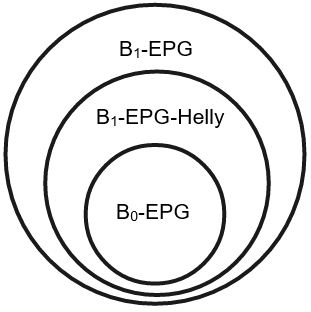
\includegraphics[width=3.5cm]{./img/diagramaClassesEPG.png}
\caption{Hierarchical diagram of some EPG classes}
\label{fig:diagramaEPG}
\end{figure}

By the results of \citep{golumbic2009}, in Lemma ~\ref{lem:representacaoC4}, every induced cycle of size 4 in a $ B_1$-EPG$(C_4)$ representation has only a possible representations.% format of a frame, true pie, or false pie, see Figure~\ref{fig:ciclotam4}.

\begin{defi} \label{defi:tortasFrame}

\citep{golumbic2009} Given a collection of paths $ P = \{p_1, \dots , p_4\}$ of a grid $ Q $ in a $ B_1-$EPG representation of the graph $ G$, consider a $ 4$-star subgraph  of $ Q $ whose center is positioned on the point $ b $ and the edges $ (a_1, b), (a_2, b), (a_3, b), (a_4, b)$ in clockwise order. We defined:

\begin{itemize}
\item A \emph{true pie} is a $ 4$-star where each segment $(a_i, b) \cup (a_ {i + 1}, b) $, to $ 1 \leq i \leq 4 $, is a different member of $ P $, where it is additionally assumed to be module 4. All 4 paths of $ G $ do bend in $ b $.

\item A \emph {false pie} is a $ 4$-star where each segment $ (a_1, b) \cup (a2, b); (a_2, b) \cup (a4, b); (a_4, b) \cup (a3, b); (a_3, b) \cup (a1, b) $, for $ 1 \leq i \leq 4 $, is a different member of $ P $. In false pie only 2 paths do not adjacent do bend in $b$.

\item Considering a rectangle of any size with 4 edges $ (x_1, y_1); (x_2, y_1); (x_2, y_2); (x_1, y_2) $. A \emph{frame} is a rectangle in which at each corner is a different bend for each member of $ p_1, \dots, p_4 \in P $. The sub-paths $ p_1 \cap p_2, p_2 \cap p_3, p_3 \cap p_4, p_4 \cap p_1 $, share at least one edge. While the sub-paths $ p_2 \cap p_4 $ and $ p_1 \cap p_3 $ do not share edge.
\end{itemize}
\end{defi}

\begin{figure}[htb]	
\center%6.3
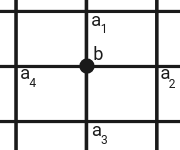
\includegraphics[width=3.5cm]{./img/centroRaioCentral.png}
\caption{Grid cut that presents center and central ray}
\label{fig:centroRaioCentral}
\end{figure}

In a $B_1$-EPG representation of a $C_4$ induced as pies where $b$ is center of the pie then there are edge-intersections $ (a_1, b), (a_2, b), (a_3, b), (a_4, b)$ called \emph{central rays}, see Figure~\ref{fig:centroRaioCentral}.

% \begin{figure}[htb]	
% \center%6.3
% 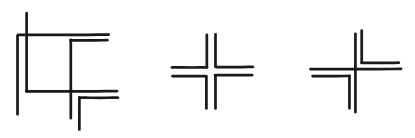
\includegraphics[width=10cm]{./img/representacaociclotam4.png}
% \caption{$B_{1}$-EPG representation of the induced cicle of size 4: frame (in left), true pie (center) and false pie (in right), \cite{golumbic2009}.}

% \end{figure}

\begin{figure}[htb]
  \centering
%segundo bloco de figuras
  \begin{tabular}{c c c c c }
    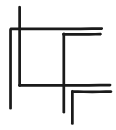
\includegraphics[width=2.3cm]{./img/representacaociclotam41.png}  
    & &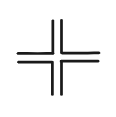
\includegraphics[width=2.5cm]{./img/representacaociclotam42.png} 
    & &
 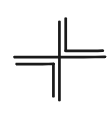
\includegraphics[width=2.5cm]{./img/representacaociclotam43.png} \\%[\abovecaptionskip]
    {\footnotesize (a) Frame}  & &  {\footnotesize (b) True pie} & & {\footnotesize (c) False pie} %\label{fig:frame}
  \end{tabular}
  \caption{$B_{1}$-EPG representation of the induced cicle of size 4}\label{fig:ciclotam4}
\end{figure} 


\begin{lema}\label{lem:representacaoC4}
\citep{golumbic2009} Every induced $C_4$  as subgraph of $ G $ corresponds, in any representation, to a true pie, false pie, or frame.
\end{lema}
\begin{proof} Given a collection of paths $ P = \ {p_1, \dots, p_4}$ of a grid $ Q $ in a $ B_1-$EPG representation of the graph $G$.

Given $ C_4 = (v_1, v_2, v_3, v_4) $ that is a chordless 4-cycle in $ G$. Given $p_i$ the path in $ G $ that corresponds to $v_i $.
Suppose $ \displaystyle \bigcap _{p_i \in P} p_i \neq \emptyset $, then clearly $ \displaystyle \bigcap _{p_i \in P} p_i = {b} $, for some point $ b $ of the grid. Since each vertex in $ C_4 $ has exactly 2 neighbors, each path $ p_i $ contains exactly two edges of the grid with end point $ b$. Thus, we obtain a star subgraph with center point $ b $ and edges $ (a_1, b), (a_2, b), (a_3, b), (a_4, b)$.
Without loss of generality, $ p_1 $ contains the edges $ (a_1, b), (a_2, b) $ of the grid. If $ p_2 $ contains $ (a_2, b), (a_3, b) $ or $ (a_1, b), (a_4, b) $, then we get a true pie. Otherwise, $ p_2 $ contains the edges $ (a_2, b), (a_4, b) $ or $ (a_1, b), (a_3, b) $ and we obtain a false pie.

Otherwise, $ \displaystyle \bigcap_ {p_i \in P} p_i = \emptyset$. Suppose $ p_1 $ is a path without bend. Each of the $ p_2 $ and $ p_4 $ paths share an edge with $ p_1 $ but do not share a common edge with any other path. If $ p_2 $ and $ p_4 $ do not have a bend, then we get a interval representation of $ C_4 - v_3 $. However, it is not possible to add a $ p_3 $ path with at most of one bend. Similarly, if $ p_2 $ and $ p_4 $ have a single bend, the $ p_3 $ path can not be added either. Therefore, $ p_1 $ has a single bend.

By symmetry, we assume that all $ p_i $ must has a single bend. Moreover, two paths can not have a bend on a common point in the grid. Thus, we obtain a rectangular subgraph with angles $ (x_1, y_1), (x_2, y_1), (x_2, y_2), (x_1, y_2) $, where $ p_1 $ bends at $ (x_1, y_1) $, $ p_2 $ bends at $ (x_2, y_1) $, $ p_3 $ bends at $ (x_2, y_2) $, and $ p_4 $ bends at $ (x_1, y_2) $, forming a frame.
\end{proof}

The \textit{octahedral} is a polyhedron that has 8 faces and it can be represented as in Figure~\ref{fig:octaedro}(a).

\begin{lema}\label{lem:octaedronaohelly}
The octahedral graph $O_3$ has a unique minimal  $ B_1$-EPG representation.%, without considering isomorphisms.
\end{lema}
\begin{proof}
The octahedral graph $ O_3 $ has in its constitution induced cycles of size 4 ($ C_4 $). The representation structures of  $ B_1$-EPG representation of $C_4$ are known in the literature and they have been previously presented.
Take an induced $ C_4 $ subgraph  any of the octahedral $ O_3 $. The two outside vertices are false twins whose neighborhood are all vertices taken for the induced $C_4$. Thus, if in a $ B_1$-EPG representation of $C_4$, the $ C_4 $ graph is represented as frame, no single bend path can be simultaneously intersecting the 4 paths representing the vertices of the induced $ C_4 $, since these paths have bends in distinct places. Therefore, we conclude that the frame structure can not be part of a $ O_3 $ representation.

With the same reasoning, take a $ B_1$-EPG representation of $C_4$ where the induced $ C_4 $ subgraph is represented as true pie or false pie. When adding the false twin vertices, which are neighbors of all vertices of $ C_4 $ taken from $ O_3 $, both representations converge to the structure represented in Figure~\ref{fig:octaedro}(b). 
\end{proof}

\begin{figure}[h]
  \centering
  
%segundo bloco de figuras
  \begin{tabular}{@{}c@{} p{3cm} @{}c@{} }
    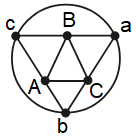
\includegraphics[width=3cm]{./img/octaedro.png} & &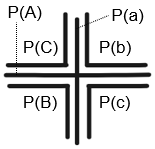
\includegraphics[width=3.5cm]{./img/representacaoOctaedro.png}  \\[\abovecaptionskip]
    \footnotesize (a) The octahedral $O_3$ graph  & &  \footnotesize(b) $B_1$-EPG($O_3$) Representation
  \end{tabular}
%  \vspace{\floatsep}
 % \begin{tabular}{@{}c@{}}
  %  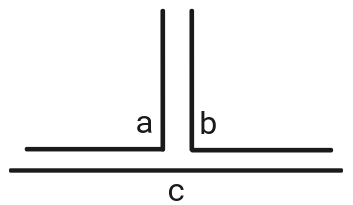
\includegraphics[width=4cm]{./img/b1epgtriangulo.png} \\[\abovecaptionskip]
  %  \small (b) Another image
  %\end{tabular}
 \caption{The octahedral $O_3$ graph and its  $B_1$-EPG representation, \cite{heldt2014}}\label{fig:octaedro}
\end{figure}

By Lemma ~\ref{lem:octaedronaohelly} the    octahedral graph $ O_3 $, from Figure ~\ref{fig:octaedro}(a), it is isomorph in any $ B_1$-EPG representation to the representation of Figure~\ref{fig:octaedro}(b). In the Figure~\ref{fig:octaedro}(b) we can see that, for example, the paths $ p(a), p(b) $ and $ p(c) $  do not satisfy the Helly property. From this observation and of the information shown in Lemma~\ref{lem:octaedronaohelly} we get the following. %Corollary~\ref{coro:b1hellyisinb1}.

\begin{coro}\label{coro:b1hellyisinb1}
%The x class is it's own subclass of the y class
The $B_1$-EPG-Helly class is properly contained in the $B_1$-EPG class.
\end{coro}

\section{$NP$-membership of $B_1$-EPG-Helly Recognition}

In this paper we will demonstrate that  $B_1$-EPG-Helly graph recognition is $NP$-complete. For this demonstration we set up a reduction from {\sc Positive (1 in 3)-3SAT} defined  as follows:

\begin{table}[h!]
\centering
%\caption{My caption}
%\label{my-label}
\begin{tabular}{ll}
\hline \hline
\multicolumn{2}{c}{\sc Positive (1 in 3)-3SAT}                                                                                                                                                                                                                                      \\ \hline \hline 
\emph{Input}: & \begin{tabular}[c]{@{}l@{}} a set $X$ of variables; a collection $C$ of clauses on $X$ where \\ for each $c\in C$, $c$ has only positive literal and $|c|\leq 3$.
\end{tabular} \\
~ & ~ \\
\emph{Goal:}  & \begin{tabular}[c]{@{}l@{}} 
Determine if there is an assignment of values to the variables in $ X $ so that \\ every clause in $ C $ has exactly one true literal.
\end{tabular} \\ \hline
\end{tabular}
\end{table}

%Um certificado para o problema {\sc Reconhecimento de grafos $B_1$-EPG-Helly} consiste em uma grade $Q$, um conjunto $P$ de caminhos em $Q$, e uma função bijetora $f$ que associa a cada vértice de $G$ um caminho de $P$ de forma que:
%\begin{itemize}
%\item para todo $e=u,v \in E(G)$ segue que $f(u)$ e $f(v)$ são intersectantes em $Q$;
%\item para todo $f(u),f(v) \in P$ tal que $f(u),f(v)$ são intersectantes em $Q$ segue que $u,v \in E(G)$;
%\item $P$ satisfaz a propriedade de Helly, i.e. todo subconjunto de caminhos mutualmente inresectantes de $P$ possui pelo menos uma aresta em comum.
%\end{itemize}

%Logo a verificação da validade de um certificado é facilmente computável em tempo polinomial, pois basta checar se $P$ satisfaz a propriedade de \textit{Helly} e forma uma $B_{1}-$EPG representação. 
%Sendo assim, no restante deste trabalho concentraremos os nossos esforços na demonstração de que o problema é NP-difícil.

% com variáveis positivas, sabidamente NP-completo, ver \citep{johnson1979}, problema [L04], página 259.

{\sc Positive (1 in 3)-3SAT } is a known NP-complete problem (see \citep{johnson1979}, problem [L04], page 259). {\sc Positive (1 in 3)-3SAT} remains NP-complete when the incidence graph of the input CNF formula is a planar graph~\citep{mulzer2008minimum}.

Given a formula $F$ of {\sc Positive (1 in 3)-3SAT} we will present a polynomial-time construction of a graph $ G_F$ such that $ G_F $ is $ B_1$-EPG-Helly if and only if $ F $ is satisfiable. This graph will contain an induced subgraph $ G_c$ with 12 vertices (called \emph {clause gadget}) for every clause $ c \in C $, and an induced subgraph (\emph {variable gadget}) containing a particular vertex  $ v_j$ for every variable $ x_j$, plus a \emph{base gadget}  with 55 additional vertices.



\section{Presentation of the problem}

In this paper we are interested in characterizing the complexity of the $B_1$-EPG-Helly recognition problem, whose formal definition is presented next:

\begin{table}[h!]
\centering
%\caption{My caption}
%\label{my-label}
\begin{tabular}{ll}
\hline \hline
\multicolumn{2}{c}{\sc $B_1$-EPG-Helly Recognition}                                                                                                                                                                                                                                      \\ \hline \hline 
\emph{Input}: & A graph $G$.\\
~ & ~ \\
\emph{Goal:}  & \begin{tabular}[c]{@{}l@{}}
Determine if there is a set of single bend paths $ P = \{p_1, p_2, \ldots, p_n\} $ \\in a grid $ Q $ %representing $ V(G) $ 
such that:\\ 
$\bullet$ \ \ \ $u,v\in V(G)$ are adjacent in $G$ if only if $p_u,p_v$ are intersecting in $Q$;\\
$\bullet$ \ \ \ $P$ satisfy the Helly propriety.
\end{tabular} \\ \hline
\end{tabular}
\end{table}



\subsection{$B_k$-EPG-Helly is in NP}

A certificate to {\sc $B_k$-EPG-Helly recognition} problem consists of $Q$, a set $P$ of paths in $Q$, and a combining function $f$ that associates each vertex in $G$ with a path  in $P$ such that:

\begin{itemize}
\item for each $e=(u,v) \in E(G)$ follow that $f(u)$ and $f(v)$ are intersecting in $Q$;
\item for each $f(u),f(v) \in P$ such that $f(u),f(v)$ are intersecting in $Q$ follow that $(u,v) \in E(G)$;
\item $P$ satisfies the Helly property, i.e. every subset of paths pairwise intersecting in $P$ has at least one common edge.
\end{itemize}

It is easy to check in polynomial time if all paths of a representation have at most $k$ bends. Thus, without loss of generality, the verification of the validity of a certificate to $B_k$-EPG-Helly recognition just needs compute in polynomial time if $ P $ satisfies the  \textit{Helly property}. This result can be achieved through a generalization of Berge's Theorem \citep{bergeDuchet1975}:

\begin{theorem} \citep{bergeDuchet1975} A hipergraph $M$ is $p$-Helly  if only if for each set $A$ of vertices with $|A| = p+1$, the intersection of the hiper-edges $E_j$ with $|E_j \cap A|\geq p$ is not empty. 
\end{theorem}

%In paper \citep{robertsSpencer1971}, the authors mention a efficient way to verify if a given family of sets satisfies the Helly property. Therefore, to verify this certificate can be computed in polynomial time. 

%Let $\mathcal{F} = \{ S_1, S_2, \dots, S_p \} $ a family of sets. Consider all triples of elements 
%The $\mathbb{F}$ family satisfy the Helly property if only if for each triple 
$ \displaystyle  u,v,w \in \mathcal{S} = \bigcup _{S_i \in \mathcal{F}} S_i$, and $\mathcal{F'}(u,v,w)$, the subfamily of all sets wich contain at least two among the elements $u,v,w$. 

%Demonstração Robert e Spencer verificação polinomial propriedade Helly
% \begin{theorem} \citep{robertsSpencer1971}
% Let $\mathcal{F} = \{ S_1, S_2, \dots, S_p \} $ a family of sets. The $\mathcal{F}$ family satisfy the Helly property if only if for each triple $ \displaystyle  u,v,w \in \mathcal{S} = \bigcup _{S_i \in \mathcal{F}} S_i$ 

% $$\bigcap \{S_i: S_i	\in \mathcal{F'}(u,v,w)\} \neq \emptyset .$$
% \end{theorem}
% \begin{proof}
% $(\Rightarrow)$ Note that the elements belonging to $\mathcal{F'}(u, v, w)$ pairwise intersect, then by hypothesis,
% $$\bigcap \{S_i: S_i	\in \mathcal{F'}(u,v,w)\} \neq \emptyset .$$
% $(\Leftarrow)$ Let $\bigcap \{S_i: S_i	\in \mathcal{F'}(u,v,w)\} \neq \emptyset$  for every triple $ \displaystyle  u,v,w \in \mathcal{S} = \bigcup _{S_i \in \mathcal{F}} S_i$.
% Suppose, by contradiction, that $\mathcal{F}$ does not satisfy the Helly property. Then there is subfamily $F_1$ of $ \mathcal{F}$ whose sets are pairwise intersecting, but there is not a common element. Consider a subset $F_2 = \{S_1, \dots, S_m\}$ a minimal subfamily of $F_1$ about  it does not satisfy the Helly property, i.e.
% \begin{itemize}
% \item $F_2$ does not satisfy the Helly property;
% \item Any subfamily with $m-1$ elements satisfies.
% \end{itemize}
% Note that $m\geq 3$. It being $F_2$ minimal about does not satisfy the Helly property, then $\bigcap _{ \mathcal{S} \in F_2-S_i	} \mathcal{S} \neq \emptyset$, for all $S_i \in F_2$. Thus,  for each $i=1, \dots, m$ there is $x_i \in (\bigcap _{j\neq i}S_j)-S_i$.
% There is $m\geq 3$, then at least three $x_i, x_j, x_k$, pairwise distinct. Thus, it being $F_2$ the minimum about does not satisfy the Helly property, each element of $F_2$ contains at least two among $x_i, x_j, x_k$.  Therefore $F_2 = \{S_1, \dots, S_m\} \subset \mathcal{F}(x_i, x_j, x_k)$, a contradiction of the our hypothesis.
% \end{proof}


\begin{lema}
For any $B_k$-EPG-Helly graph $G$ there exists  a $B_k$-EPG-Helly representation $Q$ of $G$ such that the size of $Q$ is bounded by $(k+V(G))$.

%Given a graph $G$, a polynomial grid is enough to a $B_k$-EPG(G) representation. %(A graph $G$ has at most $n(k + 1) \times n(k + 1)$ relevant edges)
\end{lema}

\begin{proof}
Consider a minimal $B_k$-EPG representation of a graph $G$, with $n$ vertices, in which the largest coordinate used (on both the $x$ and $y$ axis) is minimized (first in $y$, and then in $x$, for example), and the smallest coordinate is $\geq 1$. Let $C$ be the value of the largest $x$-coordinate.

 Therefore, all columns $1 \leq c \leq C$ is necessary for the representation, and correspond to the beginning, end, or bend of some path.

The total number of starts, ends, and bends is n(k + 1), and at most $C \leq n(k + 1)$.

The reasoning can also be applied to vertical.
\end{proof}

From now on we will go consider that we have a minimal certificate, i.e. minimized, we still consider that $k$ is polynomial on the size of the certificate. 

%Para cada tripla T de arestas da grade, seja C'  o subconjunto de caminhos de G, que contém pelo menos duas arestas da tripla T. A representação será Helly, se e somente os caminhos em cada um dos subconjuntos C', assim formados, possuírem  uma aresta em comum, para todas as triplas T.
\begin{theorem}
For each triple $T=\{u,v,w\}$ of edges of a $B_k$-EPG representation, let $\mathcal{P}=\{P_1, P_2, \dots, P_n\}$ the collection of paths relationship to vertices of the graph $G$ on grid $Q$ and $C'$ the sub-collection that contains every paths $P_i$ that have at least two edges this triple $T$. A $B_k$-EPG representation will be Helly if only if the paths in each subset $C'$ have a common edge for all triple $T$. 
\end{theorem}

\begin{proof}
$(\Rightarrow)$ Note that the paths that have edges belonging to $\mathcal{C'}(u, v, w)$ pairwise intersect, then by hypothesis,
$$\bigcap \{P_i: P_i	\in \mathcal{C'}(u,v,w)\} \neq \emptyset .$$
$(\Leftarrow)$ Let $\bigcap \{P_i: P_i	\in \mathcal{C'}(u,v,w)\} \neq \emptyset$  for every triple $ \displaystyle  u,v,w \in \mathcal{S} = \bigcup _{P_i \in \mathcal{P}} P_i$.
Suppose, by contradiction, that $\mathcal{P}$ does not satisfy the Helly property. Then there is sub-collection $C_1$ of $ \mathcal{P}$ whose sets are pairwise intersecting, but there is not a common element. Consider a sub-collection $C_2 = \{P_1, \dots, P_m\}$ a minimal sub-collection of $C_1$ about  it does not satisfy the Helly property, i.e.
\begin{itemize}
\item $C_2$ does not satisfy the Helly property;
\item Any subfamily with $m-1$ elements satisfies.
\end{itemize}
Note that $m\geq 3$. It being $C_2$ minimal about does not satisfy the Helly property, then $\bigcap _{ \mathcal{S} \in C_2-P_i	} \mathcal{S} \neq \emptyset$, for all $S_i \in C_2$. Thus,  for each $i=1, \dots, m$ there is edge $e_i \in (\bigcap _{j\neq i}P_j)-P_i$.
There is $m\geq 3$, then at least three $e_i, e_j, e_k$, pairwise distinct. Thus, it being $C_2$ the minimum about does not satisfy the Helly property, each element of $C_2$ contains at least two among $e_i, e_j, e_k$.  Therefore $C_2 = \{P_1, \dots, P_m\} \subset \mathcal{P}(e_i, e_j, e_k)$, a contradiction of the our hypothesis.
\end{proof}


\begin{coro}
{\sc $B_k$-EPG-Helly  recognition} is in $NP$.
\end{coro}
 



\section{$NP$-hardness}\label{sec:sectionDispositivoClausula}

We will use a graph $M$ isomorphic to the graph presented in Figure~\ref{fig:gadgetBase}, as a gadget to perform the demonstration. The gadget will be used in the reasoning developed from that point forward. For each  clause $c$ of a formula $F$ of the target problem, we will create a  graph $M$ (\emph{clause gadgets}), denoted by $G_c$. This gadget graph consists of subgraphs whose $B_1$-EPG representation is well known in the literature, such as: cycles of size 3 and 4 (respectively $ C_3, C_4 $).

\begin{figure}[htb]	
\center%6.3
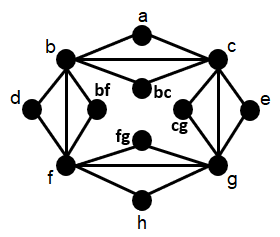
\includegraphics[width=4.5cm]{./img/gadgetBase.png}
\caption{The $H$ graph}
\label{fig:gadgetBase}
\end{figure} 

%@comment trecho retirado porque a definição entrou na seção de introdução e/ou preliminares
%Para abreviar a escrita, por abuso de notação e para efetuar uma padronização no texto será utilizada a notação $B_{k}$-EPG$(G)$ para denotar uma representação $B_{k}$-EPG do grafo $G$, onde $k$ é o número máximo de dobras que cada caminho possui nessa representação EPG de $G$. Analogamente, utilizaremos a notação $M$-$B_{k}$-EPG$(G)$ para denotar uma representação $B_{k}$-EPG do grafo $G$ que satisfaz a propriedade Helly.

\begin{defi}
\label{lab:lab1}
Let $M$ be the graph shown in Figure~\ref{fig:gadgetBase}. We denote by \emph{center} of a $B_1$-EPG representation of $M$ such that $M[\{b, c, f, g \}]$ is represented as false pie or true pie, the unique grid-point of this representation in which is contained in every path representing the vertices in $ \{b, c, f, g \}$.
\end{defi}

\begin{defi}\citep{golumbic2009}
Let $M$ be the graph shown in Figure~\ref{fig:gadgetBase}. In each $B_1$-EPG representation of $M$, where $M[\{b, c, f, g \}]$ is represented as false pie or true pie, we denote by \emph {central ray} the edge-intersection  between two paths of $ \{b, c, f, g \} $ starting from the center.
\end{defi}

Note that every $B_1$-EPG representation of a $C_4$ satisfies the Helly property, and triangles have $B_1$-EPG representations that satisfy the Helly property, e.g. the one shown in Figure~\ref{fig:triangulos}(b). The graph $M$ is composed by a $C_4^M=M[b, c, f, g]$ and for eight cycles of size 3, which are $(a,b,c);$ $(b,c,bc);$ $(c,e,g);$ $(c,g,cg);$ $(f,g,h);$ $(f,g,fg);$ $(b,d,f);$ $(b,f,bf).$

Like $C_4^M$ has a finite number of known representations, shown in Figure~\ref{fig:ciclotam4}, then we can start drawing the $B_{1}$-EPG-Helly representation of $M$ from these structures. The Figures~\ref{fig:falsepietruepieframe}(a), ~\ref{fig:falsepietruepieframe}(b) and ~\ref{fig:falsepietruepieframe}(c) present 3 possibilities of representation of graph $M$, except for isomorphisms. The frame structure has characteristics different than the pies, which makes it less intuitive to understand, so we will make a more detailed discussion about the $B_1$-EPG representation of the frame structure in Section~\ref{subsec:moldura}.

If $C_4^M$ is represented by pie, then the paths $p(b), p(c), p(f), p(g)$ share a central point of the representation. But if $C_4^M$ is represented by a frame, then the bends of the 4 paths corresponding to the four distinct corners of a rectangle, i.e. all path representing a vertex of $C_4^M$ has a distinct bend point, see~\citep{golumbic2009}.

As every vertex of $M$ has exactly two neighbors in $C_4^M $, then all paths in a $B_1$-EPG representation of $M$ are intersecting a pair of paths in the $B_1$-EPG representation of $C_4^M$. In this way, there will be exactly two paths that intersect each pair of central rays, see Figures~\ref{fig:falsepietruepieframe}(a) e~\ref{fig:falsepietruepieframe}(b). 

\subsection{The special case of the frame structure} \label{subsec:moldura}

Because asymmetric representations, the frame structure needs to be studied in more detail. Next we will show some constraints of this structure in which allow us to use it as gadget in the demonstration.

\begin{prop}\label{lem:direcoesdiferentes}
In any $B_1$-EPG representation of a $C_4$ as frame every path $p_i$ that represents a vertex of the $C_4$ intersects exactly two other paths of the frame $p_{i-1}$ and $p_{i+1}$, where one of them is vertical and another is a horizontal intersection.
\end{prop}

\begin{proof}
Let a $B_1$-EPG representation of a $C_4$ as frame where $P = \{p_1, \dots, p_4\}$ is the collection paths of this representation.  Every paths have a bend and they have one part in the vertical and another part in the horizontal, by  definition in~\citep{golumbic2009}. Suppose there is a path $p_i$ of the frame that connects two other paths $p_{i-1} $ and $ p_{i + 1}$, both horizontally. Then we have that $p_i, p_{i-1}$ and $ p_{i + 1}$ have bend over the same straight line. But, by frame definition, these bend points should be the corners of a rectangle, a contradiction.
\end{proof}

\begin{prop}\label{lem:mesmaretasuporte}
Given a $B_1$-EPG-Helly representation of a graph, where the representation of a $C_4$ is isomorphic to a frame, if there is a vertex $v$ of $G$, outside this $C_4$, that is adjacent to exactly two consecutive vertices of this $C_4$, then the path representing $V$ shares at least one common edge-intersection with the both paths representing neighbors of $V$ into such $C_4$.  
\end{prop}

\begin{proof}
Given $p_1$ and $p_2$ paths that represent consecutive vertices of the $C_4$, in a representation isomorphic at frame, and $B_1$-EPG-Helly such that $p_1 \cap p_2 \neq \emptyset$.
Suppose that exist a third path, $p_x$, adjacent to $p_1$ and $p_2$, but $p_x \cap (p_1 \cap p_2) = \emptyset$. If this situation occurs, then the structure does not can be  Helly, a contradiction.
\end{proof}

%\cleardoublepage

By Proposition~\ref{lem:direcoesdiferentes} and Proposition~\ref{lem:mesmaretasuporte} we can conclude that for every vertex $v_i \in V(M)$ such that $v_i \neq V(C_4^M)$, when we use frame to a $B_{1}$-EPG-Helly representation of the $C_4^M$, $p(v_i)$ will have at least one common edge-intersection to a pair of paths equivalent to its neighbor vertices of $M$. Then, in the Figure~\ref{fig:falsepietruepieframe}(a), Figure~\ref{fig:falsepietruepieframe}(b) and Figure~\ref{fig:falsepietruepieframe}(c) are presented some possible $B_{1}$-EPG-Helly representation of $M$. On every $B_{1}$-EPG-Helly representation presented we can apply rotation and mirroring operations, because these operations do not alter the edge intersecting representation structure.


\begin{prop}
Em qualquer representacao $B_{1}$-EPG-Helly do grafo $M$ os seguintes pares de caminhos sao colineares na sua parte que está conectada à representação do $C_4^M$ : $p(a)$ e $p(bc)$; $p(e)$ e $p(cg)$; $p(h)$ e $p(fg)$; $p(d)$ e $p(bf)$.
\end{prop}

\begin{lema}
Os caminhos $p(a), p(e), p(d)$ e $p(h)$ estao obrigatoriamente 2 na direcao vertical e 2 na direcao horizontal.
\end{lema}



%\begin{figure}[htb]
  \centering
%segundo bloco de figuras
  \begin{tabular}{c c c c c }
    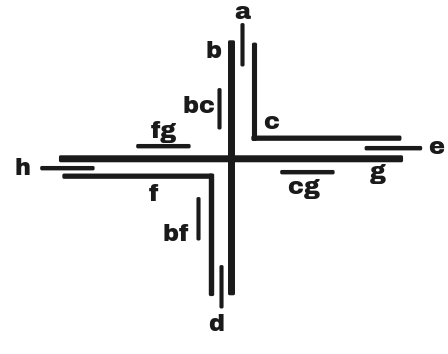
\includegraphics[width=4cm]{./img/falsePie.png}  %\label{fig:falsePie} 
    & &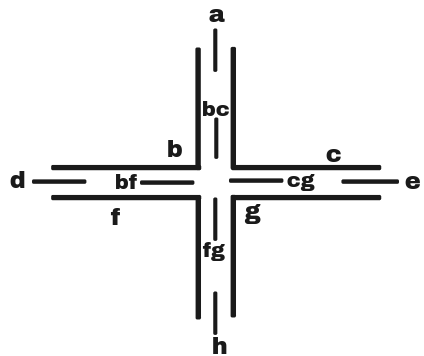
\includegraphics[width=4cm]{./img/truePie.png} %\label{fig:truePie}
    & &
 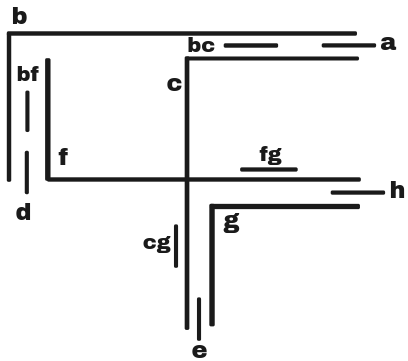
\includegraphics[width=4cm]{./img/frame.png} \\%[\abovecaptionskip]
    {\footnotesize (a) Based in false pie}  & &  {\footnotesize(b) Based in true pie} & & {\footnotesize (c) Based in frame} %\label{fig:frame}
  \end{tabular}
  \caption{Differents representations in single bend of the $H$ graph, see Figura~\ref{fig:gadgetBase}, according with structure used to represent the $C_4^H$}\label{fig:falsepietruepieframe}
\end{figure} 

%Perceba que nas representações $B_{1H}(G_c)$, tanto elas sendo representadas como tortas ou quanto representadas como moldura, cada aresta indicando adjacência entre dois vértices de $G_c$ possui intersecção com outras duas arestas (não adjacentes entre si) que representam, obviamente, os dois vértices adjacentes a cada par de vértices do $C_4$ no grafo $G_c$.

\begin{figure}[htb]
  \centering
%segundo bloco de figuras
  \begin{tabular}{c c c c c }
    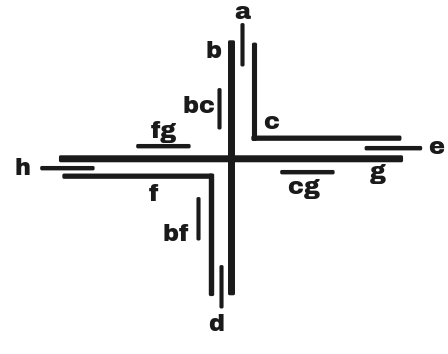
\includegraphics[width=4cm]{./img/falsePie.png}  %\label{fig:falsePie} 
    & &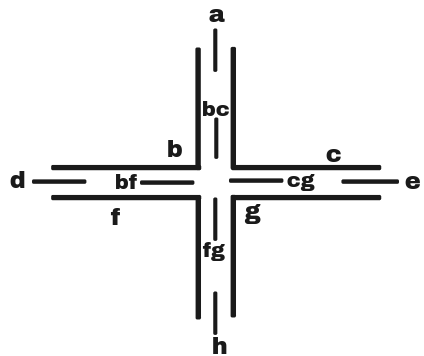
\includegraphics[width=4cm]{./img/truePie.png} %\label{fig:truePie}
    & &
 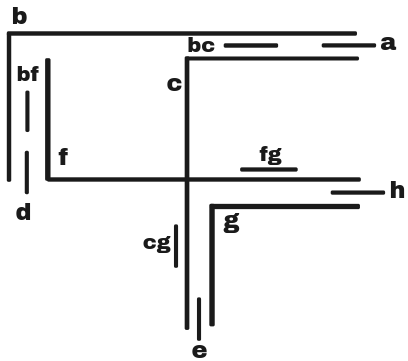
\includegraphics[width=4cm]{./img/frame.png} \\%[\abovecaptionskip]
    {\footnotesize (a) Based in false pie}  & &  {\footnotesize(b) Based in true pie} & & {\footnotesize (c) Based in frame} %\label{fig:frame}
  \end{tabular}
  \caption{Differents representations in single bend of the $H$ graph, see Figura~\ref{fig:gadgetBase}, according with structure used to represent the $C_4^H$}\label{fig:falsepietruepieframe}
\end{figure} 

%Agora que conseguimos representar nosso \textit{dispositivo} base com um formato de razoável controle, podemos partir para a construção da cláusula \textit{dispositivo}. Denotaremos por $G_{C}$ o \textit{dispositivo} que irá representar a cláusula. Esse grafo é uma construção sobre $G_c$. Para obter $G_{C}$ são adicionados 8 vértices em $G_{C}$ da seguinte forma: 4 vértices, denotados $x_i$, para $1\leq i \leq 4$ são adjacentes a cada um dos três vértices de cada um dos 4 triângulos mais externos mostrados em $G_{C}$, onde $i$ vai representar o $i-$ésimo triângulo externo ao qual $x_i$ se conecta. O vértice $y_i$ vai se conectar a dois dos vértices da vizinhança de $x_i$, onde, obrigatoriamente, um desses vértices não faz parte do $C_4$ induzido e o outro faz, sem perda de generalidade e por convenção tomemos o par mais a adiantado em sentido horário, como mostrado na Figura~\ref{fig:dispositivoBaseClausula}.   

%Como $G_{C}$ é supergrafo de $G_{C}$ então faz sentido aproveitarmos as representações $B_{1H}(G_B)$ para montarmos a representação $B_{1H}(G_c)$. Ao final da inserção, os vértices adicionados estão em destaque com cor diferente.

%\input{./includes/include-img/gadgetB1EpgHellyClausulas.tex}

%\input{./includes/include-img/representacoesB1EpgHellyClausula.tex}


%\input{./includes/include-img/representacoesB1EpgHellyClausula2.tex}


% @comment

\begin{lema}\label{lem:obstrucao}
Given a graph $ G'$ consisting of a vertex $ x $, two isomorphic graphs at $ M $, they are $ H_1 $ and $ H_2 $, and a bipartite graph $ K_{2,4}$, where: $ x $ is a vertex of the largest stable set of $ K_{2,4} $; $x $ is adjacent to an induced cycle of size 3 of $ H_1 $, $ C_3^{H_1} $; $x $ is also adjacent to another induced cycle of size 3 of $ H_2 $, $ C_3^{H_2}$, see Figure~\ref{fig:extremidadeDobraObstruida}(a). In a single bend representation the ends path and the bend of $p(x) $ are obstructed.%, i.e. another path $ p(q) $ can not be intersecting only the $ p(x) $ by the ends of the path nor by the bend.
\end{lema}

\begin{proof}
In any single bend representation of $ G'$ the following happens. Since $ p(x) $ is part of the largest stable set in $ K_{2,4} $ then the paths belonging to the largest stable set always will do bend into a false pie, more details in \citep{Asinowski2009}, then $ p(x) $ has a condition of \emph {obstructed bend}, see Figure~\ref{fig:extremidadeDobraObstruida}. Since $ p(x) $ is adjacent to $ C_{3}^{H_1}$ and $ C_3^{H_2}$, then $ p(x) $ must be adjacent to both paths representing these triples of vertices. For the Lemma~\ref{lem:mesmaretasuporte} and Figure~\ref{fig:falsepietruepieframe} we can note that adjacent to any pair of paths of $ C_4^M $ there are two non-intersecting paths. Considering that only one of the two triples of vertices that share the same edge pair of $ C_4^M $ is adjacent to $ p(x) $, this implies that $ p(x) $ has a condition of \emph{obstructed extreme}, see Figure~\ref{fig:extremidadeDobraObstruida}.
\end{proof}

\begin{figure}[h]
  \centering
  \begin{tabular}{p{5cm} p{1cm} p{5cm}}
     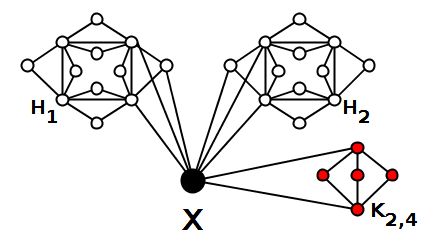
\includegraphics[width=5cm, center]{./img/grafoDobraExtremidadeObstruida.png} & &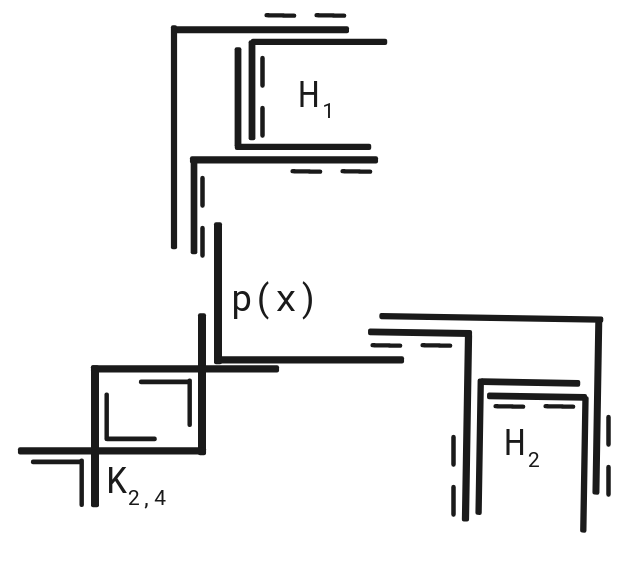
\includegraphics[width=5cm, center]{./img/extremidadeDobraObstruida.png}  \\%[\abovecaptionskip]
    \footnotesize \centering (a) The $G'$ graph& & \footnotesize \centering (b)A $B_1$-EPG$(G')$ representation%\\
 %   &&
  \end{tabular}
 \caption{The sample of obstruction far end and obstruction bend}\label{fig:extremidadeDobraObstruida}
\end{figure}

-> Considere o grafo da Figura 9 (a), se adicionarmos um novo vertice y adjacente somente ao vertice x, então na B1-EPG representacao desse grafo o caminho p(y) possui um segmento maximal dominado por p(x). Isso significa que o segmento maximal de p(y) que é adjacente a p(x) estah totalmente contido em algum segmento de p(x), e ainda como p(x) possui dobra e extremidades obstruidas entao isso implica que o segmento maximal p(y) que eh adjacente a p(x) tambem estah obstruido.

-> Duvida 1: inserir aqui tambem a parte que diz que se esse vertice y for adjacente a um outro vertice z entao obrigatoriamente y terah que possuir uma dobra?

-> Duvida 2: Se a duvida anterior for incluida, entao posso incluir a situacao em que esse vertice y possui tambem suas mais dois elementos de obstrucao adjacentes a ele o que implica que alem do segmento maximal adjacente a p(x) tambem o segmento perpendicular (de dobra) tambem esta obstruido.  


\subsection{The problem reduction}\label{sec:reducao}

The reduction of a formula $F$ from  {\sc Positive (1 in 3)-3SAT}  to a particular graph $G_F$ that will have  $B_{1}$-EPG-Helly representation of $G_F$, if only if $F$ is satisfactory, it is given below.

\begin{enumerate}
\item For each clause $C_i \in F$ there is a  \textit{clause gadget} $G_{c}$, isomorph to $M$ graph, that can be draw in single bend and Helly, as in same representation of the Figures~\ref{fig:falsepietruepieframe}(a), ~\ref{fig:falsepietruepieframe}(b) or~\ref{fig:falsepietruepieframe}(c)  ;

\item For each variable $x_{j}$ there is a vertex $v_{j}$ that is adjacent to $a$, $e,$ or $M$, vertices of $G_c$, when $x_{j}$ is the first, second or third variable in $C_i$, in this order;

\item For each vertex $v_{j}$, are added 2 isomorphic graphs  at $M$, $H_1$ and $H_2$, where $v_{j}$ is  adjacent to a triangle ((a,b,c); (c,e,g); (g,f,h); or (b,d,f)) of each $H_1$ and $H_2$; 

\item The induced subgraph by \emph{pivot vertex}  $v_{j}$, and also $V(H_1)$ and $V(H_2)$ will be called \emph{variable gadget}; 

\item There is a vertex $V$, that will be used as vertical reference of the construction, adjacent to each vertex  $d \in V(G_c)$;

\item There is a bipartite graph $K_{2,4}$ with a particular vertex $T$ that is in the largest stable set. This vertex is nominated \emph{true vertex}. $T$ is adjacent to all $v_{j}$ and also to $V$;

\item There are two isomorphic graphs at $M$, $G_{B1}$ and $G_{B2}$. The vertex $T$ is connected to a triangle between ((a,b,c); (c,e,g); (g,f,h); or (b,d,f)) of each;


\item There are two isomorphic graphs at $M$, $G_{B3}$ and $G_{B4}$. The vertex $V$ is connected to a triangle between ((a,b,c); (c,e,g); (g,f,h); or (b,d,f)) of each;

\item The induced subgraph by vertices $V(K_{2,4})$, $T$ and $V$,  $V(G_{B_1})$ and $V(G_{B_2})$, and also $V(G_{B_3})$ and $V(G_{B_4})$ will be nominated as \emph{base gadget}. 
\end{enumerate}


The Figure~\ref{fig:exemploGrafoGF} represents the graph that would be obtained when the previous construction is applied to the formula $ F = (x_1 + x_2 + x_3) \wedge (x_2 + x_3 + x_4) \wedge (x_1 + x_3 + x_4) $, on {\sc Positive (1 in 3)-3SAT}. %, the graph $ G_F $ will be like in the Figure~\ref{fig:exemploGrafoGF}.
 Consider that we can assign the following values to variables that will satisfy the formula $F$: $x_1 = False; x_2 = False; x_3 = True; x_4 = False$. Thus, considering this assignment we can have a $B_1$-EPG representation similar to the Figure~\ref{fig:grafoFormula}.


\begin{figure}[htb]	
\center%6.3
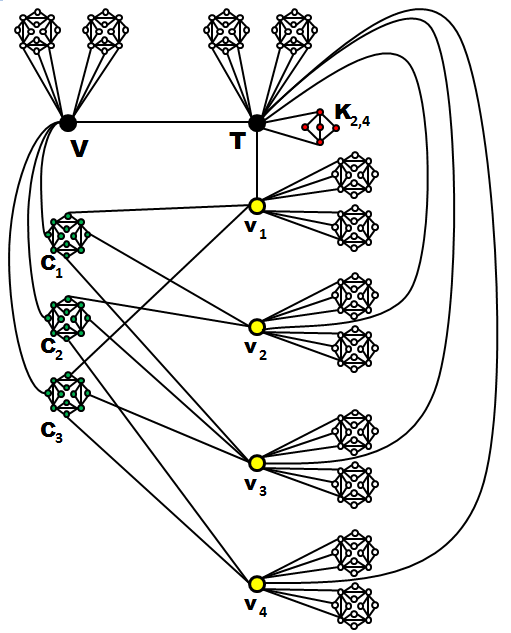
\includegraphics[width=8cm]{./img/exemploGrafoGFSBPO3.png}
\caption{The $G_{F}$ graph to formula $F=(x_1+ x_2+ x_3) \wedge  (x_2+ x_3+ x_4 )\wedge  (x_1 + x_3+ x_4 )$}
\label{fig:exemploGrafoGF}
\end{figure}

\begin{figure}[htb]	
\center%6.3
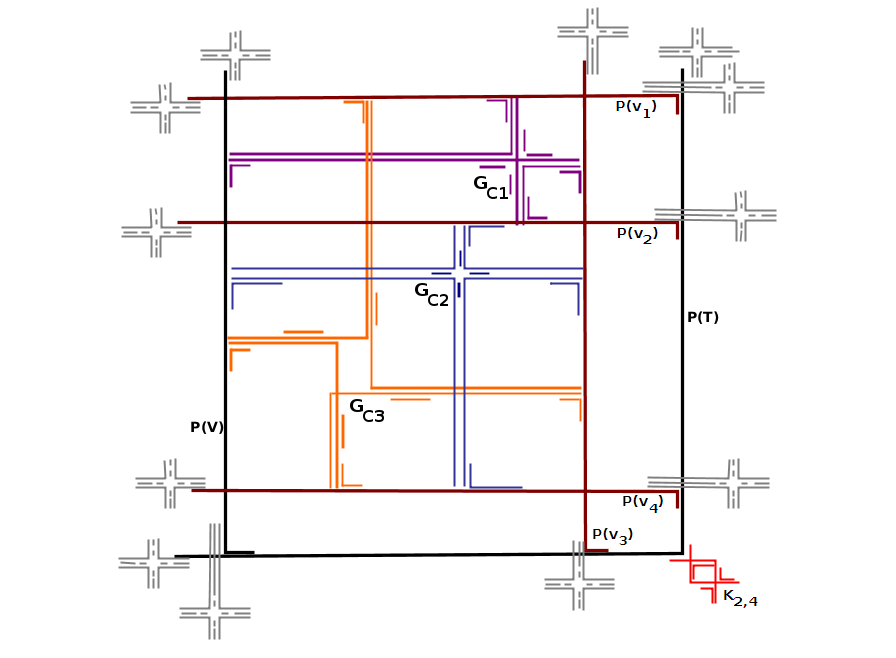
\includegraphics[width=1\textwidth]{./img/formulaGFCompletaSBPO3diferentes2.png}
\caption{The $B_{1}$-EPG-Helly representation to gadget $G_{F}$ of the Figure~\ref{fig:exemploGrafoGF}.%, to formula $F=(x_1+ x_2+ x_3) \wedge  (x_2+ x_3+ x_4 )\wedge  (x_1+ x_3+ x_4 )$. 
 The gadget's clause $G_{c_1}$ represented by false pie, the gadget's clause $G_{c_2}$ represented by true pie, and the gadget's clause $G_{c_3}$ represented by frame.}
\label{fig:grafoFormula}
\end{figure}


First, we construct a minimal single bend representation for the base gadget, including the vertices $T$ and $V$. Such a representation, will be used as a base to guide as the representation of each clause gadget (i.e. $B_1$-EPG representation of $G_{c_i}$), is inserted in the structure. %The representations of the vertices that correspond to the variables of the formula (i.e. each $p(v_i)$), are also inserted according to the order that appear in the clause and value that each variable can assume.

%@comment retirado para SBPO
%A seguir, serão apresentadas as regras para efetuar as ligações no modelo $B_1$-EPG-Helly, i.e. uma $B_{1}$-EPG-Helly${(G_F)}$. Observe uma construção parcial dessa representação  na Figura~\ref{fig:clausulagadgetgf} que mostra uma representação de fórmula satisfatível.

%@comment retirado para SBPO
\begin{figure}[htb]	
\center%6.3
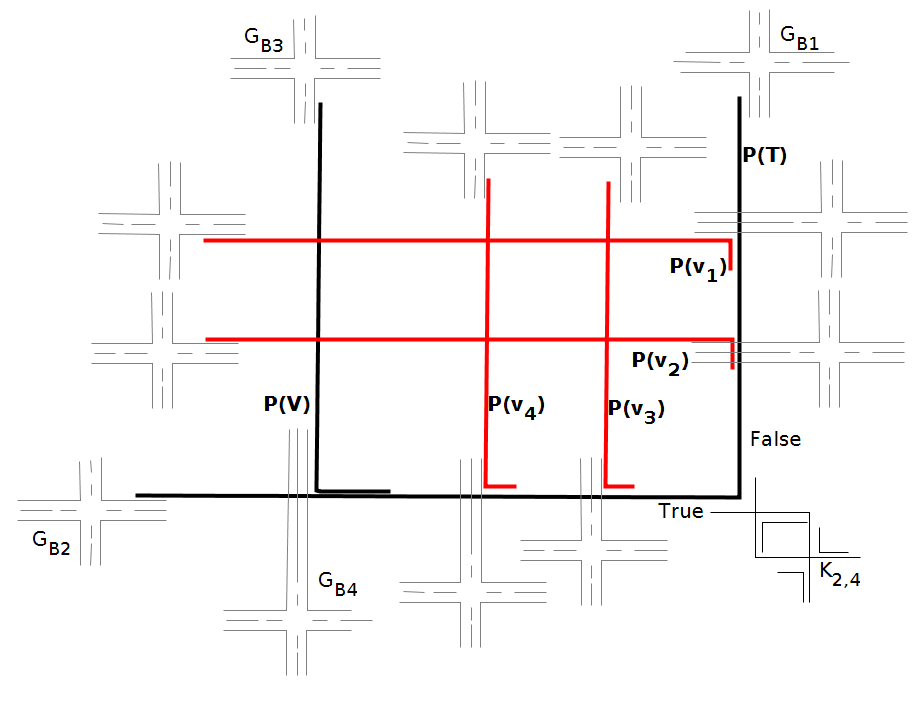
\includegraphics[width=10cm]{./img/gradeb1epghellySBPO.png}
\caption{Single bend and Helly representation of the forumla $F'$, no clause gadgets}
\label{fig:gradeb1epg}
\end{figure}

\begin{theorem}
The $B_{1}$-EPG-Helly graph recognition is NP-hard.
\end{theorem}

\begin{proof}
Given an instance $F$ of {\sc Positive (1 in 3)-3SAT} we construct a graph $G_F$ as previously described. We will show that $G_F$ has a   $B_{1}$-EPG-Helly representation if only if $F$ is satisfiable.

$(\Rightarrow)$ Suppose that $G_F$ has a $B_1$-EPG-Helly representation, $R_{G_F}$. Without loss of generality assume that $p(V) \cap p(T)$ is a horizontal segment in  $R_{G_F}$. From $R_{G_F}$ we will construct an assignment that satisfies $F$ as follows: assign for each variable $ x_{j}$ true value if the edge intersecting $p(v_j)$ and $p(T)$ is horizontal, and false otherwise.

Note that every single bend representation of a $K_{2,4}$ graph, the path of each vertex of the greater stable set, in particular $p(T)$ here represented, it has bend in a false pie, see \citep{Asinowski2009}. This condition forces $p(T)$ to bend in a false pie of $B_1$-EPG representation of $K_{2,4}$. 

The vertex $T$ is adjacent to vertices in a external triangle of $G_{B1}$ and $G_{B2}$. As the $K_{2,4}$ is positioned in the bend of $p(T)$, thus in any $B_{1}$-EPG-Helly representation of $G_{B1}$  and of $G_{B2}$, they are positioned at the ends of $p(T)$, or together to bend, see Lemma~\ref{lem:obstrucao}.   

If a single bend Helly representation of the \textit{clause gadget} has as base the true or false pie, there are two triple of edges on the same line support. This block the clause gadget from positioning in an intermediate part of  $p(T)$, i.e. it has to be allocated in a end, explanation can be found in the section~\ref{sec:sectionDispositivoClausula}. By Lemma~\ref{lem:mesmaretasuporte}, we know that whether the base of the representation of the clause gadget it is a frame, a third vertex  adjacent to edge-intersection of a $C_4$ must share at least one these intersection segments. Thus, since there are two vertices in the \textit{clause gadget}  that share same neighborhood, at least one segment of each path of both vertices is on the same line support, which block the frame from having a completely contained side in a true vertex path $p(T)$. Thus, also in this case the clause gadget will be positioned at the end of the path of $p(T)$.

As we take the adjacency between $p(V)$ and $p(T)$ horizontally, then any edge intersection in $p(V)$, with the exception of $p(T)$, obviously is vertical. Since $V$ is adjacent to vertices of the more external triangles in $G_{B3}$ and $G_{B4}$, the two vertical ends of the segments of $p(V)$ are obstructed by $G_{B3}$ and $G_{B4}$, respectively. Thus, the vertical segment of the path $p(d_{c_i})$ to each \textit{clause gadget} is completely contained in the vertical segment of $p(V)$.At that moment, the horizontal segments of each $p(d_{c_i})$, they must be positioned  to bending and to adjacency with $p(V)$. Consequently, if the $C_4^M$ of each clause gadget $G_c$ is  represented by a true pie or false so, the another three center ray, two are verticals and one is horizontal. If the $C_4^M$ of the \textit{clause gadget} $G_c$ is represented by a  \textit{frame},as frame has 4 distinct bends, where each path that is in $C_4^M$ is positioned in one of these bends, so always that $p(d_{c_i})$ is horizontal segment, also there will be two segments that are verticals and only one other path that is also horizontal (among $p(a_{c_i}),p(e_{c_i}), p(h_{c_i})$), otherwise the structure do not is a  \textit{frame}, see Lemma~\ref{lem:direcoesdiferentes}. The consequence of this structure, both for pies and frame is that this generates that in all \textit{clause gadget} the edege-intersection among only two $\{p(a_{c_i}), p(e_{c_i}), p(h_{c_i})\}$ and each $p(v_{j})$ are two horizontal and exactly one is vertical. In other words, every clause contains exactly one true variable.

In any assignment the paths represented by $p(a_{c_i}), p(e_{c_i}), p(h_{c_i})$ have make bend to that there is intersection with $p(v_{j})$. Each \textit{variable gadget} has a pivot vertex  $p(v_{j})$ and two isomorphic graphs to $M$ with one more external triangle adjacent to $v_j$, as previously explained, these isomorphic graphs $M$, they must they can only connect at one end or bend of a path. Therefore, as the $p(v_{j})$ already does  adjacency with $p(T)$ then one of its ends is obstructed. It is then left to position the isomorphic to $M$ at the other end and in the bend of that path. In this way, any other vertex that is connected to   $p(v_{j})$ must connect in a do not extreme intermediate space. We conclude that $p(v_{j})$ is bend and end obstructed. 

As the segments $p(a_{c_i}), p(e_{c_i}), p(h_{c_i})$ are two in vertical position and one  in horizontal position. Assuming $p(a_{c_i}), p(e_{c_i}), p(h_{c_i})$ can not connect to the paths of the variables by the ends, since these are already occupied. Whereas, furthermore,by Lemma~\ref{lem:mesmaretasuporte} and by definition of pies, $p(a_{c_i}), p(e_{c_i}), p(h_{c_i})$ do not can be completely contained in some $p(v_j)$ in the same direction as him. So necessarily, $p(a_{c_i}), p(e_{c_i}), p(h_{c_i})$ must connect to two paths of variables with false assignment (that connect vertically to
 $p(T)$) and to a variable path with true assignment. Otherwise there would not be $R_{G_F}$.


$(\Leftarrow)$ Given an assignment that satisfies $F$, we can construct $R_{G_F}$. First we represent all structure of the base gadget and the variable gadget, related to  $G_{F}$, with exception  \textit{clause gadgets},
%@comment retirado para o SBPO
%, como apresentado na Figura~\ref{fig:gradeb1epg}, 
this construction must respect the restrictions presented in subsection~\ref{sec:reducao}. 

A path $p(v_{j})$ is connected to path $p(T)$, by true vertex $T$, horizontally, if $x_{j}$ is true and vertically if $x_{j}$ is false. 

%~\ref{fig:representacaoCaminhos}
Without loss of generality and for simplicity in explanation, we will use the true pie and false pie structures to represent $ G_C$, but the construction could also be done with the frame structure (the Figure~\ref{fig:grafoFormula} presents the clause gadgets as false pie, true pie and frame). 

To insert a \textit{ clause gadget} $G_{C}$, we introduce an imaginary horizontal line $l_{h}$ in the grid between the horizontal lines used by the paths for the two false variables in $ C $. Then we connect the way $p(d_{c_i})$ of $G_{C}$ in $p(V)$ vertically using the bend of $p(d_{c_i})$. However, we introduce a vertical imaginary line $ l_{v}$ in the grid, between the vertical line of the grid used by $p(V)$ and the path to the true variable in $C_j$, i.e. between $p(V)$ and the path of the true variable $x_i \in C_j$. Where $l_{h}$ and $l_{v}$ cross, to insert the center of the  \textit{clause gadget} as can be seen in Figure~\ref{fig:clausulagadgetgf}. 

There is a permutation that we can represent all the settings for  $p(a_{c_i})$, $p(e_{c_i})$ e $p(h_{c_i})$, using pies, with $p(d_{c_i})$ fixed, these permutations are presented in the Figure~\ref{fig:disposicoes}. In other words,  it is possible to represent all combinations of assignments where the vertices $p(a_{c_i})$, $p(e_{c_i})$ and $p(h_{c_i})$ are relationship to variables with a assignment satisfiable. %Quando fixamos o $p(d)$, está ilustrado na 
The Figure~\ref{fig:clausulagadgetgf} illustrates a provision for the relationship among the  $p(a_{c_i})$, $p(e_{c_i}), $ and $p(h_{c_i}) $, and variables with values $False$,  $True$, $False$, respectively.  

\begin{figure}[h!]
\centering
% \subfloat [Representação de Torta Falsa]{\includegraphics[width=12cm]{./img/representacaoFalsePieGadgetClausula.png}\label{fig:falsePie}}
% \qquad
 \subfloat[$p(e), p(a), p(h)$ adjacent to variables with values $False, True,False$, respectively]{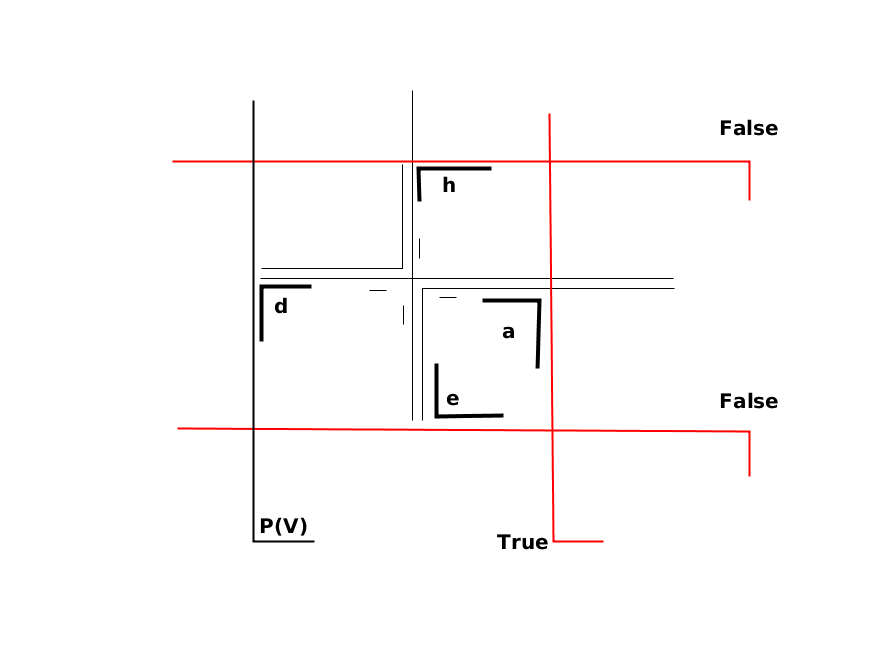
\includegraphics[width=7.8cm]{./img/clausulaGadgetDisposicoesefathf.png}\label{fig:disposicao1}}
 %\qquad
\subfloat[][ $p(e), p(a), p(h)$ adjacent to variables with values $False,False, True$, respectively]{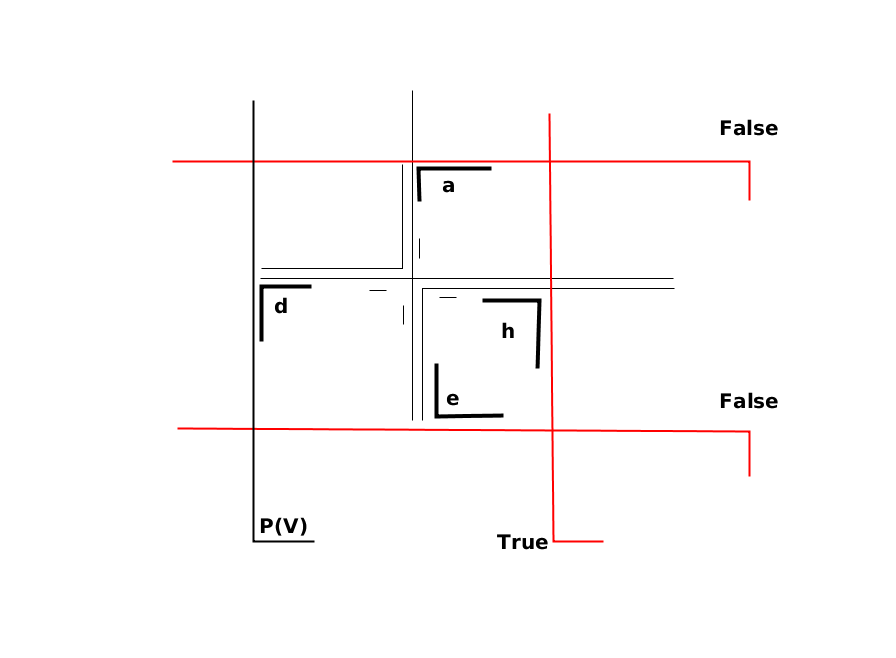
\includegraphics[width=7.8cm]{./img/clausulaGadgetDisposicoesefafht.png}\label{fig:disposicao2}}
\caption{Representation to differents variable arrangements, using structure of false pie.}
\label{fig:disposicoes}
\end{figure}  
  

\begin{figure}[htb]	
\center%6.3
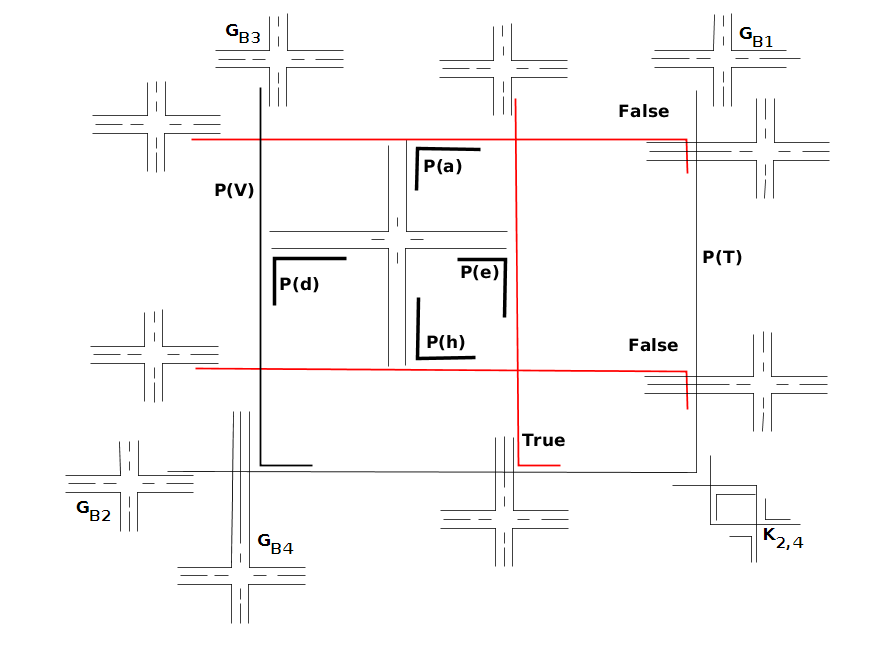
\includegraphics[width=8cm]{./img/clausulaGadgetGFCompletaSBPO.png}
\caption{Clause gadget positioned in a assignment satisfiable.}
\label{fig:clausulagadgetgf}
\end{figure}


Note also that the single bend representation of the base gadget that we use respects the Helly property for the edges. Likewise, the single bend  representation of the clause gadget also respects the Helly property. Furthermore, the single bend representation of the set of vertices of the variable gadget respects the Helly property. And when we join all these representations of subgraphs in the graph of the formula $ G_F $, it also has a representation $ B_1$-EPG that respects the Helly property, when $ F $ is satisfiable.

%~\ref{fig:representacaoCaminhos}

%Devido ao fato de T se conectar aos vértices de um triângulo mais externo ((a,b,c); (c,e,g); (g,f,h); (b,d,f)) da cláusula \textit{dispositivo} base $G_c$, e como em qualquer representação $B_1-$EPG-Helly de $G_c$ esse triângulo comparilha vértices com outro triângulo mais interno ((b,c,bc);(c,g,cg);(f,g,fg);(b,f,bf)), então, 


Thus we show that a formula $F$ in {\sc Positive (1 IN 3)-3SAT }, is satisfiable if only if there is a $R_{G_F}$.
\end{proof}



\bibliographystyle{sbpo}
\bibliography{exemplo-latex}



\end{document}

